% =====================================================================
%  Capítulo 12 — Puntos a golpear
% =====================================================================
\chapter{Puntos a golpear}

El daño producido por un golpe en partes específicas donde el organismo es más vulnerable es mucho mayor que en cualquier otro punto al azar. Estos puntos se denominan \enquote{puntos vitales}, no porque su ataque determine la muerte instantánea, sino porque el efecto es muy superior al de las zonas vecinas. Lograr un golpe definitivo es bastante difícil: dependen de la resistencia corporal, la potencia, la técnica, el equilibrio y el movimiento. Recuerda el marco legal: estos recursos se justifican por la necesidad racional de interrumpir una agresión, no para prolongarla.

Estas regiones pueden atacarse con golpes o con presiones de dedos. Es recomendable familiarizarse con ellas presionando suavemente en el propio cuerpo hasta ubicar el lugar exacto de sensibilidad. Intentaremos golpear: espacios intermusculares y sistema nervioso periférico, arterias y venas, órganos huecos, articulaciones, músculos y huesos.

\section{Los puntos más accesibles con técnicas simples}

\begin{itemize}
  \item \textbf{Ojos:} muy sensibles; pueden atacarse con la punta de los dedos y objetos punzantes, presionarse contra el borde orbitario, o usarse para distracciones (arrojar tierra, llaves o un simple amago) que regalan el segundo necesario para atacar o huir.
  \item \textbf{Entrecejo:} aloja el hueso etmoides, esponja ósea muy vascularizada; su fractura (con elementos contundentes) provoca gran hemorragia. La frente, en cambio, es de las zonas más duras: golpearla con el puño puede fracturarnos la mano.
  \item \textbf{Nariz:} su fractura provoca dolor y lagrimeo; el golpe con la base de la palma es seguro para nuestra mano.
  \item \textbf{Boca:} su rotura es muy invalidante, pero no debe atacarse con la mano desnuda (riesgo de heridas e infección por mordedura), sino con objetos o con el codo.
  \item \textbf{Oídos:} sensibles al impacto con la palma abierta (\enquote{sopapo} que aumenta la presión y lesiona el tímpano).
  \item \textbf{Laringe y garganta:} muy susceptible a golpes; atacarla puede provocar desmayo e incluso la muerte: reservar para peligro extremo.
  \item \textbf{Clavículas:} se buscan fracturas con golpes tipo \enquote{martillo} del puño o con elementos contundentes para incapacitar el brazo.
  \item \textbf{Dedos de las manos:} clave para romper agarres (hasta del pelo): toma cualquier dedo y haz palanca para hiperextenderlo.
  \item \textbf{Manubrio del esternón:} metiendo un dedo en el hueco sobre el esternón y empujando hacia atrás y abajo se gana distancia (probar suavemente en el propio cuerpo).
  \item \textbf{Plexo solar:} golpearlo afecta a la red nerviosa abdominal y provoca incapacitación temporal.
  \item \textbf{Genitales:} efecto similar al anterior; se atacan con patada en distancia larga, rodillazo en la corta o agarre/apretón en el cuerpo a cuerpo.
  \item \textbf{Rodilla:} se ataca con patadas (punta o tacón del zapato sobre la rótula) para reducir la movilidad. Los golpes bajos son rápidos, difíciles de detener y crean sorpresa para enlazar otra técnica.
  \item \textbf{Tibia:} patear de frente su cara interna (sin musculatura) provoca dolor agudo; de espaldas, con el talón, sirve contra agarres por detrás.
  \item \textbf{Empeine y dedos de los pies:} pisotones de frente o con el tacón hacia atrás para liberarse de agarres; su fractura puede definir un enfrentamiento al impedir la movilidad.
\end{itemize}

\newpage

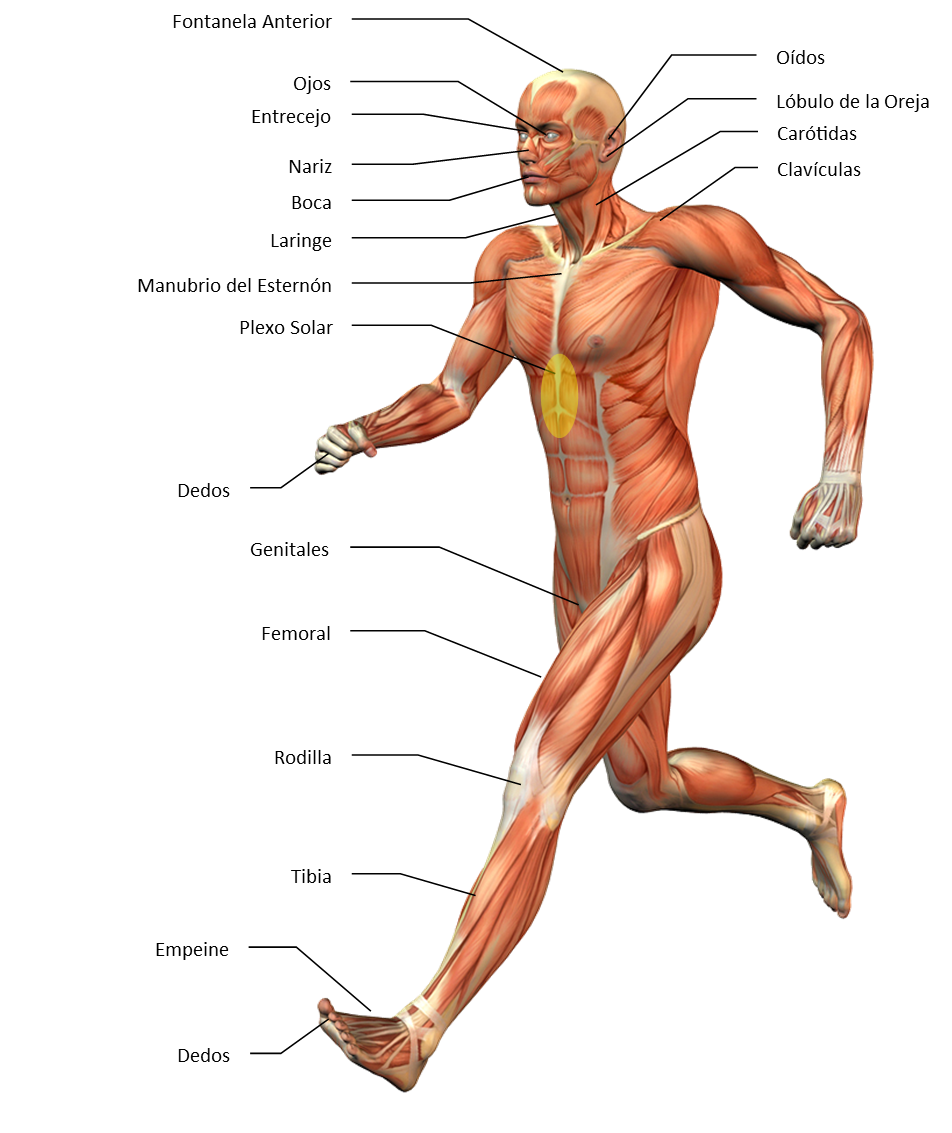
\includegraphics[width=\linewidth]{figures/Imagen8.png}
